\section{The model}
\label{sec:dsmc_model}
DSMC is a model that makes full use of statistical mechanics the kinetic theory of gases. The physical system consists of $N$ atoms in a box with volume $V$ and porosity $\phi$ (the porosity was the fraction of the total volume available for fluids). Instead of tracking the trajectory every single atom, we simulate $M$ particles, each representing $N_\text{eff}$ real atoms. We can interpret this approximation as that all atoms in a small region of space around the coordinates of a simulated particle move with approximately the same velocity. The state of a DSMC simulation is fully described by $6M$ phase variables, three velocities and three positions per simulated particle. Since we don't have detailed information about the positions of all the real atoms, we don't calculate the forces between the particles. Instead, we assume that the gas particles only undergo binary collisions (we neglect collisions between three or more particles), just like we did while deriving the Boltzmann equation in section \ref{sec:boltzmann_equation}. Collisions are performed in a stochastic manner, where the rate of collisions and post-collision velocities are determined from kinetic theory. We can think that the collision step in the model is an operator, or a stochastic function $\mathcal{C}(\vec r, \vec v, \mathcal{G})$, where $\vec r$ and $\vec v$ form the phase space point and $\mathcal G$ contains all information about the system geometry. Don't worry, this will be clear in a minute.\\
The equations of motion are integrated by applying the standard Euler method on the positions so that $\vec r_i(t+\Delta t) = \vec r_i(t) + \vec v_i(t)\Delta t$ for particle $i$. The timestep is chosen small enough so that we can split it into two parts; moving and colliding. This is a reasonable assumption as long as the timestep $\Delta t$ is smaller than the mean collision time $\tau_{coll}$ (equation \eqref{eq:kinetic_theory_mean_collision_time})
\begin{align}
	\Delta t \leq \tau_{coll} = \frac{1}{\sqrt 2 \pi \sigma^2 \rho_n \langle v \rangle},
\end{align}
since the velocity then is a constant during the timestep. If a particle interacts with a boundary during the timestep, some sort of surface interaction rule is applied before the timestep is continued (we allow a particle to collide with the surface several times during a single timestep). The moving step can also be seen as a stochastic operator, $\mathcal{M}(\vec r, \vec v, \mathcal{G})$. The operator is clearly dependent of the position $\vec r$, velocity $\vec v$ and the geometry $\mathcal{G}$. Different surface interaction models are discussed in section \ref{sec:surface_interactions} with a detailed description of the implementation in section \ref{sec:dsmc_complex_geometries}. Statistical properties are sampled at the end of each timestep where the physical quantities are sampled as time averages. A flow chart illustrating the steps of a typical DSMC algorithm is presented in figure \ref{fig:dsmc_flowchart}.
\begin{figure}[ht]
\begin{center}
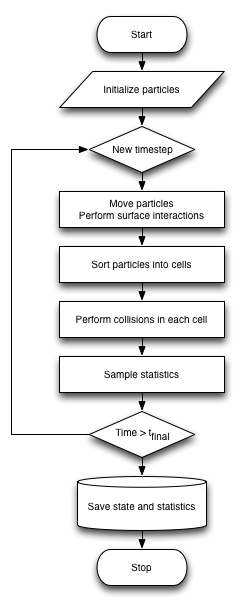
\includegraphics[width=\textwidth, trim=0cm 0cm 0cm 0cm, clip]{DSMC/figures/dsmc_flowchart.png}
\end{center}
\caption{Typical steps for a DSMC algorithm.}
\label{fig:dsmc_flowchart}
\end{figure}

\section{Collisions}
\label{sec:dsmc_collisions_model}
In a particle simulation with a continuous force field it is not clear how one would define a \textit{collision event}. If two equal atoms with the same velocity move towards each other, the atoms would at some point reverse their velocity. In this case, one could define the collision event to occur at the time when their relative distance is at its minimum, but other equally valid definitions probably exists. It is however clear that a collision should be identified as an event that happens when the atoms are close, i.e. short ranged forces. In this model, we have chosen the \textit{hard sphere} model, where each particle is assumed to be a perfect hard sphere with diameter $d$ and mass $m$. Hard sphere means that two particles with radius $R_1$ and $R_2$ will undergo an elastic collision if their relative distance equals the sum of their radii, see figure \ref{fig:dsmc_hard_sphere}. In DSMC, we will apply what we could call a stochastic hard sphere collision model, where we use the hard sphere model only to calculate the statistical collision rates. We only want nearby particles to collide, so we sort the particles into spatial cells, allowing only particles from the same cell to collide. The dimension of these cells should not exceed the mean free path. If this was the case, two particles displaced by a distance larger than a mean free path could transfer momentum or energy faster than what would happen in a real gas. Note that we allow particles moving away from each other collide, since the simulated particles should not be interpreted as real molecules or atoms. In some sense, they are quasi-particles carrying statistical information only.
\begin{figure}[h]
\begin{center}
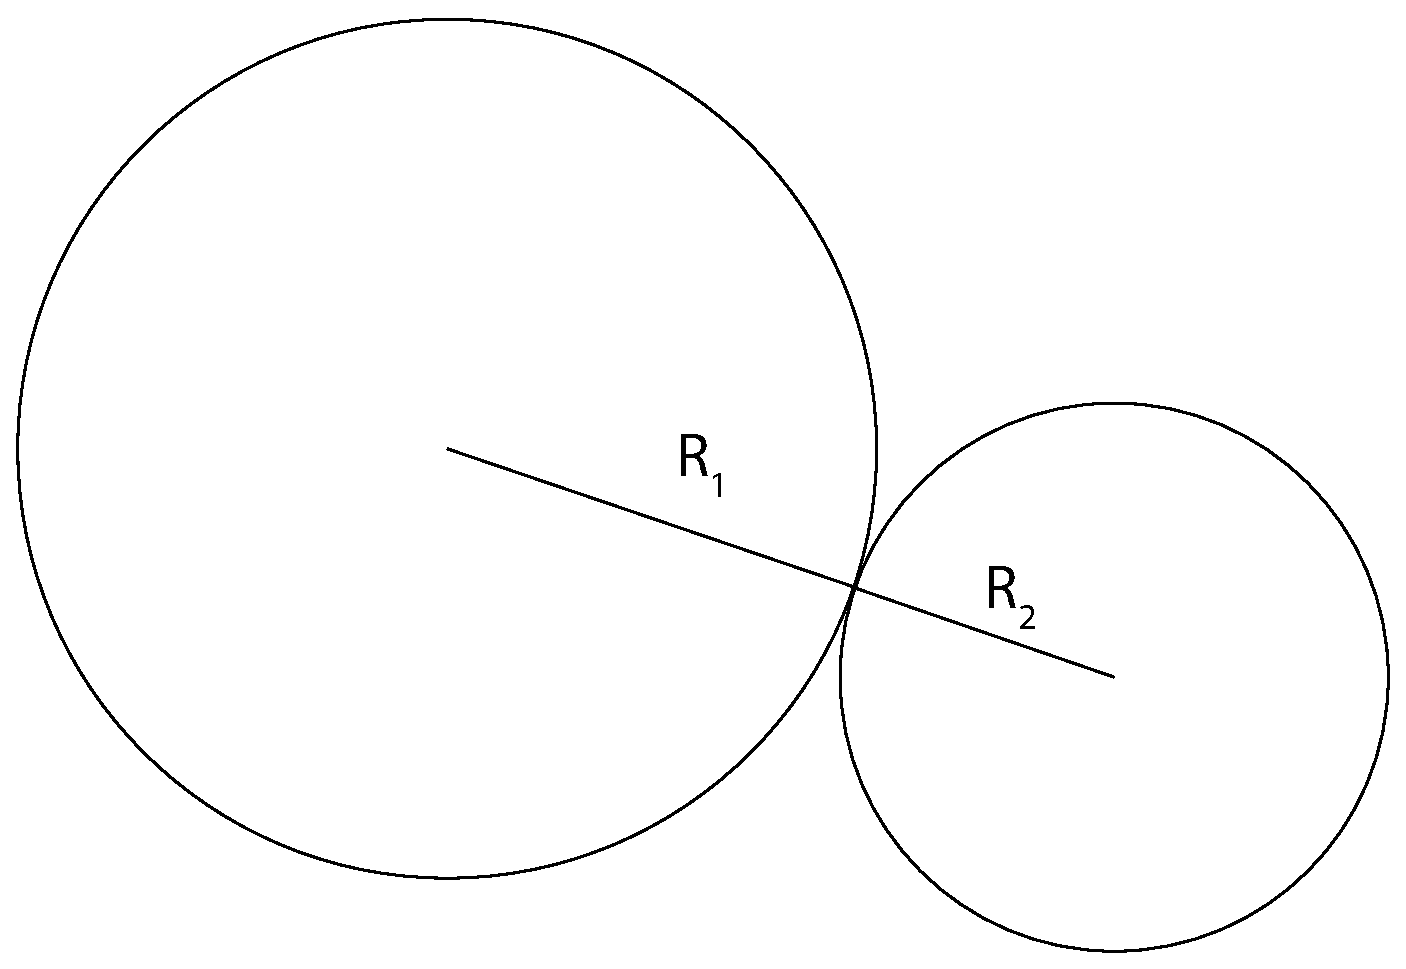
\includegraphics[width=0.5\textwidth, trim=0cm 0cm 0cm 0cm, clip]{DSMC/figures/collisions.eps}
\end{center}
\caption{The hard sphere collision model. Two particles will collide if their relative distance becomes smaller than $R_1+R_2$.}
\label{fig:dsmc_hard_sphere}
\end{figure}
\subsection{Number of collisions}
If we select two particles $i$ and $j$ with relative velocity $\vec v_r$ and cross section $\sigma=\pi d^2$, each representing $N_\text{eff}$ real atoms in a cell with volume $V_c$, the total volume sweeped out during a timestep is
\begin{align}
	V_\text{sweep} = N_\text{eff}\sigma^2|\vec v_r|\Delta t.
\end{align}
The probability of collision is the total sweeped volume $V_{sweep}$ divided by the total cell volume $V_c$
\begin{align}
	P = {N_\text{eff}\sigma^2|\vec v_r|\Delta t \over V_c}.
\end{align}
For each particle, there are $N-1$ potential collision partners. So the total number of collision pairs (we divide by two to prevent double counting of pairs) is $N(N-1)/2$ which gives the number of collisions $M_\text{coll}$
\begin{align}
	M_\text{coll} = {N(N-1)N_\text{eff}\sigma^2\langle v_r \rangle \Delta t\over 2 V_c},
\end{align}
where we replaced the relative velocity $v_r$ by the mean value in the cell
\begin{align}
	\langle v_r \rangle = {1\over N} \sum_{i\neq j} |\vec v_i - \vec v_j|.
\end{align}
Instead of calculating the mean relative velocity in each cell every timestep, we instead calculate $M_\text{cand}$ collision \textit{candidate pairs} so that
\begin{align}
	{M_\text{coll}\over M_\text{cand}} = {\langle v_r\rangle \over v_r^\text{max}},
\end{align}
since the probability of collision is proportional to the relative velocity. Each of these candidates go through an acceptance-rejection process where we pick a uniform random number $\mathcal{R}_1\in (0,1)$ and accept the collision if
\begin{align}
	v_r \leq v_r^\text{max}\mathcal{R}_1.
\end{align}
This will only accept $\langle v_r\rangle/v_r^\text{max}$ of the candidates and we end up with $M_\text{coll}$ actual collisions, as desired. Note that even particles that move away from each other can collide. This property has, as we will see in section \ref{sec:dsmc_eos}, an interesting consequence leading to which equation of state the gas satisfies.
\subsection{Post-collision velocities}
After a collision is accepted, we want to choose new velocities conserving both energy and momentum. We need a total of six equations to determine the post-collision velocities where four are provided through the conservation laws. Conservation of momentum yields that the center of mass velocity is unchanged
\begin{align}
	\vec v_\text{cm} = \frac{1}{2}(\vec v_i + \vec v_j) = \frac{1}{2}(\vec v_i^* + \vec v_j^*) = \vec v_\text{cm}^*,
\end{align}
where the energy conservation tells us that the relative velocity vector does not change its magnitude
\begin{align}
	v_r = |\vec v_i - \vec v_j| = |\vec v_i^* - \vec v_j^*| = v_r^*.
\end{align}
Here we used that $\vec v_i\cdot\vec v_j = 0$ on average since they are uncorrelated. The two remaining degrees of freedom are determined by choosing the direction of the relative velocity
\begin{align}
	\vec v_r^* = v_r\left[(\sin\theta\cos\phi)\vec i + (\sin\theta\sin\phi) \vec j + (\cos\theta)\vec k\right],
\end{align}
where the angles are uniformly distributed over the unit sphere so that all directions for the relative velocity are equally probable. The area element $\dm\Omega$ can be written as
\begin{align}
	\dm\Omega = \sin\theta \dm\theta \dm\phi = -\dm\phi \dm(\cos\theta),
\end{align}
so we need to choose $\phi$ and $\cos\theta$ uniformly. This is easy, we simply choose 
\begin{align*}
	\phi = 2\pi\mathcal{R}_2 & \qquad \qquad \cos\theta = 2\mathcal{R}_3 - 1,
\end{align*}
where $\mathcal{R}_2$ and $\mathcal{R}_3$ are random numbers in the range $(0,1)$ and we calculate $\sin\theta = \sqrt{1 - \cos^2\theta}$. The post-collisions velocities are then found by
\begin{align}
	\vec v_i^* = \vec v_\text{cm} + \frac{1}{2}\vec v_r^*\\
	\vec v_j^* = \vec v_\text{cm} - \frac{1}{2}\vec v_r^*.
\end{align}
An example of how this can be implemented is found in listing \ref{lst:post_collisions_velocities}.
\begin{lstlisting}[caption=Determining post-collision velocities., label=lst:post_collisions_velocities]
void collide_molecules(Vector3 &v0, Vector3 &v1, Random *rnd) {
    Vector3 v_center_of_mass = 0.5*(v0 + v1);
    double relative_velocity_magnitude = (v1 - v2).length();
    
    double cos_theta = 1.0 - 2.0*rnd->next_double();
    double sin_theta = sqrt(1.0 - cos_th*cos_th);
    double phi = 2*M_PI*rnd->next_double();

    Vector3 relative_velocity(1,1,1)*relative_velocity_magnitude;
    relative_velocity.x *= cos_theta;
    relative_velocity.y *= sin_theta*cos(phi);
    relative_velocity.z *= sin_theta*sin(phi);
    v0 = v_center_of_mass + 0.5*relative_velocity;
    v1 = v_center_of_mass - 0.5*relative_velocity;
}
\end{lstlisting}
